\label{sec:database-structure}
The database was designed in a way that keeps
generation or storage of redundant information at a minimum. The complete
structure diagram of the database is shown in Figure \ref{fig:dbstructure} (page
\pageref{fig:dbstructure}). All tables, except the ``ests'', ``hmmsearch'', and
``blast'' tables, are used to store information about the amino acid or
nucleotide sequences that belong to either an ortholog set or a proteome of a
reference taxon, or both. 

All tables have an ``id'' column with an auto-incremented integer as a unique
identifier. This identifier is used in specialized queries that reference other
tables. 

The database is structured ``from inside out'': the core data are the reference
proteomes. All record relationships are derived from them. They are stored in
the table ``aaseqs'' as amino acid sequences. If nucleotide sequences from the
corresponding set of protein-coding genes are present, they are stored in the
table ``ntseqs''. What nucleotide sequence corresponds to what amino acid
sequence is stored in the table ``sequence\_pairs''. The proteome and annotated
set of protein-coding genes are commonly referred to and published as ``official
gene set'' (OGS).  Multiple OGS versions of
the same species can be stored concurrently; they are distinguished by their
version number in the database, which is stored in the table ``ogs'' and
referenced by the column ``ogs\_id'' in the table ``sequence\_pairs''.  All
sequence records and the sequence\_pairs couples are referenced to a taxon
ID. The taxon information is stored in the table
``taxa''.  OGS data can be of either nucleotide or amino acid sequences; the
sequence type column is referenced to the table ``types'', which has only two
records---``nt'' for nucleotide and ``aa'' for amino acid sequences---and serves
as a labeling table.

A subset of the genes contained in the reference proteomes can be classified
into ortholog groups. This relationship is reflected in the database: the table
``orthologs'' holds the necessary information to construct clusters of ortholog
groups; each group is tagged with an identifier and references the table
``sequence\_pairs'', where the sequences in question are in turn referenced.
Each ortholog group is part of an ortholog set, which is detailed with a
shorthand name and a description in the table ``set\_details''.

Data that are relevant to a specific analysis, \eg, assessing orthology in a
specific query transcriptome library, are stored in the tables ``ests'',
``hmmsearch'', and ``blast''.  The first table contains the transcriptome
sequence data from a query species.  This table, like the other tables that
contain sequence data, has a column that specifies a taxon ID as well as a
column that specifies a sequence type.

The tables that contain sequence data, \ie, ``aaseqs'', ``ntseqs'', and ``ests''
also have a column that holds a user ID. The table ``users'' can be referenced
to identify a username. This was introduced to connect the uploading of an amino
acid or nucleotide sequence dataset to a specific user in order to facilitate
separation of multiple datasets by different researchers in the same database.

In the table ``hmmsearch'', the results of the HMM search are located. This
table also has a column that specifies a taxon ID, but it stores no amino acid
or nucleotide sequence data. Instead, it records \emph{references} to the
sequences in question. This practice helps avoid redundant storage of nucleotide
or amino acid sequence data, which can take up valuable space on the hard drive.
Frequently, not an entire amino acid sequence is part of a best hit during a HMM
search, but only a particular domain, \ie, a subsequence. This is reflected by
storing the start and end of the hit in the respective columns. 

The table ``blast'' is similarly structured to the table ``hmmsearch'': it, too,
stores only references to amino acid sequence records that were hit by a BLAST
search, and defines the start and end of the hit subsequence.

Using this database structure, it is possible to construct specialized SQL
queries to retrieve specific information, \eg, all amino acid sequences that
belong to a given ortholog set (see \autoref{fig:db-orthoset} for this example),
or all clusters of ortholog candidates. The different \pname programs
extensively rely on this database structure. They are explained in the following
section.

\begin{figure}[h]
	\centering
	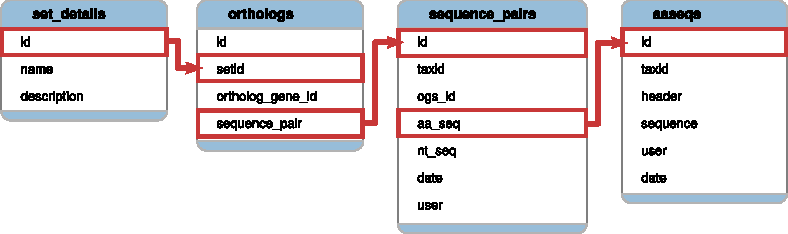
\includegraphics{img/db-orthoset.pdf}
	\caption[Database table connections for a given ortholog set]{
		\pname database structure for a given ortholog set. Each rounded rectangle
		represents a table with named columns. The red path delineates the
		\code{JOIN} query structure that returns all amino acid sequences (stored in
		the table ``aaseqs'') that belong to a given ortholog set. Ortholog set
		information is stored in the table ``set\_details''.
	}
	\label{fig:db-orthoset}
\end{figure}


\begin{figure}[ht]
	\centering
	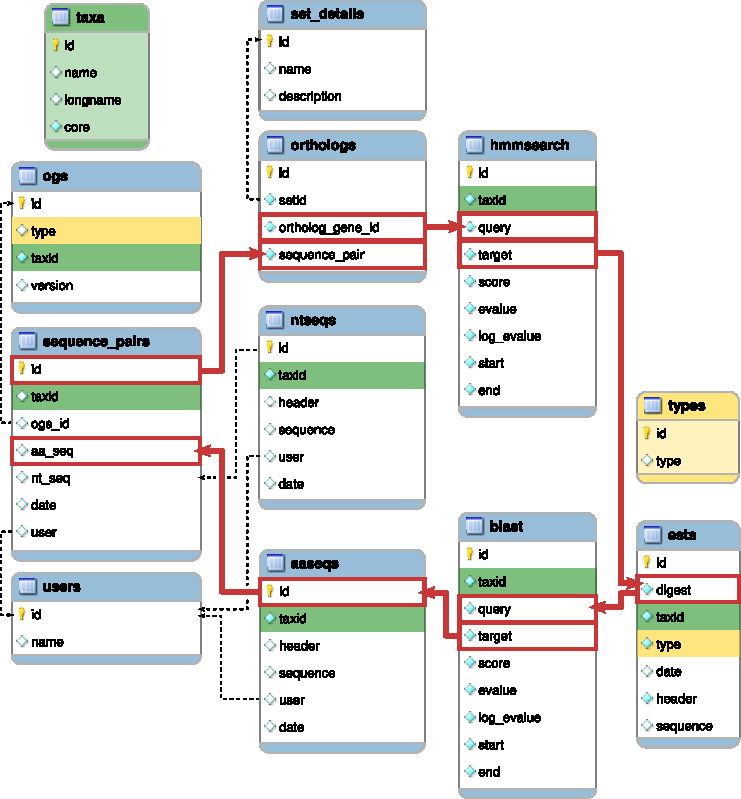
\includegraphics[width=\textwidth]{img/dbstructure.pdf}
	\caption[\pname database structure]{
		\pname database structure. Each rectangle represents a table with named
		columns. Note the circular path (red) that can be drawn across the tables and
		that is used in \code{JOIN} queries in order to construct a graph of
		orthologous relationships. Green table columns are referenced to the ``taxa''
		table, and yellow table columns are referenced to the ``types'' table. Dotted
		lines are secondary references.
	}
	\label{fig:dbstructure}
\end{figure}



